%% FullCourse_10Lecs -- Lecture 10, Topic 10.6a: Case Study 5 --- Inside the Sprint (Setup)
%% Source: ./archive_pre_split/Lec10_Case_Studies_v2.tex (section 6, first half)
%% Pre-emptive sub-split: section 6 has ~50 frames so it is split into T6a (Setup) + T6b (Execution).
%% Split point: line 2034 of source (end of Stage 1; next sectiondivider opens Stages 2, 3, 4).
%% T6a covers: opening Case 5 sectiondivider, Case 5 vs Case 4, four-day timeline,
%%             four-stage arc, six-element template, Acts 1--5 of Stage 1.
%% FullCourse-only content (Case 5 Sprint not in MiniCourse).

%% Shared preamble for the FullCourse_10Lecs topic decks.
%%
%% Each topic .tex \input's this file, then defines its own \title, \date
%% override (if any), \graphicspath, and \begin{document}.
%%
%% Reconstructed verbatim from the inlined copy preserved in
%% Lec10_Case_Studies/Lec10_T8_Case6_DeepRamsey.tex (lines 23-190), which is
%% explicitly annotated there as "from ../shared_preamble.tex, copied verbatim".
%% Base preamble matches MiniCourse_8hr/Slides/shared_preamble.tex; this version
%% additionally provides \sectiondivider, the conceptbox/cautionbox/examplebox/
%% takeawaybox tcolorboxes, and \compacttables used across the split decks.

\documentclass[10pt,english,aspectratio=169]{beamer}

\usepackage{ae,aecompl}
\usepackage[T1]{fontenc}
\usepackage{textcomp}
\usepackage[utf8]{inputenc}
\usepackage{babel}
\usepackage{datetime2}

\setcounter{secnumdepth}{3}
\setcounter{tocdepth}{3}

\usepackage{amsmath, amssymb, amsthm, graphicx}
\usepackage{booktabs, multirow}
\usepackage{tikz}
\usepackage{pgfplots}
\pgfplotsset{compat=1.16}
\usepackage[most]{tcolorbox}
\tcbuselibrary{skins, breakable, theorems}
\usepackage{listings}
\usepackage{xcolor}

\lstset{
  basicstyle=\ttfamily\small,
  keywordstyle=\color{blue!80!black}\bfseries,
  commentstyle=\color{green!50!black}\itshape,
  stringstyle=\color{orange!80!black},
  backgroundcolor=\color{gray!8},
  frame=single,
  rulecolor=\color{gray!40},
  breaklines=true,
  showstringspaces=false,
  numbers=none,
}

\lstdefinestyle{pythonstyle}{
    language=Python,
    basicstyle=\ttfamily\footnotesize,
    keywordstyle=\color{blue!80!black}\bfseries,
    commentstyle=\color{green!50!black}\itshape,
    stringstyle=\color{orange!80!black},
    frame=single,
    breaklines=true,
    showstringspaces=false,
    numbers=left,
    numbersep=5pt,
    numberstyle=\tiny\color{gray},
    backgroundcolor=\color{gray!8},
    rulecolor=\color{gray!40}
}

\ifx\hypersetup\undefined
  \AtBeginDocument{%
    \hypersetup{bookmarks=false,breaklinks=true,pdfborder={0 0 0},colorlinks=true,
      linkcolor=DarkText,urlcolor=RedTitle}%
  }
\else
  \hypersetup{bookmarks=false,breaklinks=true,pdfborder={0 0 0},colorlinks=true,
    linkcolor=DarkText,urlcolor=RedTitle}%
\fi

\makeatletter
\newcommand\makebeamertitle{%
  \begin{frame}[plain]
    \vspace*{1.0cm}
    \centering
    {\usebeamerfont{title}\usebeamercolor[fg]{title}\inserttitle\par}
    \vspace{1.0cm}
    {\usebeamerfont{author}\usebeamercolor[fg]{author}\insertauthor\par}
    \vspace{0.2cm}
    {\usebeamerfont{date}\usebeamercolor[fg]{date}\insertdate\par}
  \end{frame}}%
\AtBeginDocument{%
  \let\origtableofcontents=\tableofcontents
  \def\tableofcontents{\@ifnextchar[{\origtableofcontents}{\gobbletableofcontents}}
  \def\gobbletableofcontents#1{\origtableofcontents}%
}

\usetheme{metropolis}
\usefonttheme{professionalfonts}

\definecolor{LightGray}{RGB}{230,230,230}
\definecolor{RedTitle}{RGB}{0,0,200}
\definecolor{VeryLightGray}{RGB}{245,245,245}
\definecolor{DarkText}{RGB}{0,0,0}

\setbeamercolor{background canvas}{bg=white}
\setbeamercolor{title}{fg=RedTitle}
\setbeamercolor{author}{fg=DarkText}
\setbeamercolor{date}{fg=DarkText}
\setbeamercolor{frametitle}{bg=VeryLightGray,fg=DarkText}
\setbeamercolor{normal text}{fg=DarkText}
\setbeamerfont{title}{size=\large}

\setbeamersize{text margin left=5mm, text margin right=5mm}
\addtobeamertemplate{frametitle}{}{\vspace{-0.5em}}
\newcommand{\reducevspace}{\vspace{-0.5cm}}

% Shared section divider and box styles for split topic decks.
\newcommand{\sectiondivider}[2]{%
\begin{frame}[plain,noframenumbering]
\begin{center}
\vfill
{\Large\textbf{#1}\par}
\vspace{0.35cm}
{\normalsize #2\par}
\vfill
\end{center}
\end{frame}
}

\newtcolorbox{conceptbox}[1][]{
  colback=blue!3,
  colframe=RedTitle!55,
  boxrule=0.35mm,
  arc=1mm,
  left=2mm,
  right=2mm,
  top=1mm,
  bottom=1mm,
  #1
}
\newtcolorbox{cautionbox}[1][]{
  colback=red!3,
  colframe=red!50!black,
  boxrule=0.35mm,
  arc=1mm,
  left=2mm,
  right=2mm,
  top=1mm,
  bottom=1mm,
  #1
}
\newtcolorbox{examplebox}[1][]{
  colback=green!3,
  colframe=green!45!black,
  boxrule=0.35mm,
  arc=1mm,
  left=2mm,
  right=2mm,
  top=1mm,
  bottom=1mm,
  #1
}
\newtcolorbox{takeawaybox}[1][]{
  colback=VeryLightGray,
  colframe=RedTitle!55,
  boxrule=0.35mm,
  arc=1mm,
  left=2mm,
  right=2mm,
  top=1mm,
  bottom=1mm,
  #1
}
\newcommand{\compacttables}{\renewcommand{\arraystretch}{1.15}}

\setbeamertemplate{navigation symbols}{}
\setbeamertemplate{footline}{%
  \hfill%
  \usebeamercolor[fg]{page number in head/foot}%
  \usebeamerfont{page number in head/foot}%
  \insertframenumber\,/\,\inserttotalframenumber\kern1em\vskip2pt%
}

\makeatother

\author{Zhigang Feng}
% "date with time": compile timestamp so each build is identifiable.
\date{\today\ \DTMcurrenttime}


% Suppress redundant auto-generated metropolis section page; \sectiondivider frames are the dividers we keep.
\metroset{sectionpage=none}

\graphicspath{{./pic/}{./figures/}{./Exercise10_ES_Fellows/plots/}{../../MiniCourse_8hr/Slides/Module4_Agentic_AI/pic/}{../}}

\usetikzlibrary{positioning,arrows.meta,shapes,calc,fit,backgrounds}

\lstdefinestyle{markdownstyle}{
    basicstyle=\ttfamily\footnotesize,
    frame=single,
    rulecolor=\color{gray!40},
    backgroundcolor=\color{gray!8},
    breaklines=true,
    showstringspaces=false,
    numbers=none,
}

\title[AI for Econ Research]{AI for Economic Research: Dynamic Models, Language, and Agents\\
Lecture 10.6a: Case Study 5 --- Inside the Sprint (Setup)}

\begin{document}

\makebeamertitle

%=============================================================================
\begin{frame}{Topic 10.6a Agenda}
\begin{enumerate}
  \item \textbf{Inside the Sprint --- Setup} --- problem framing, environment setup, early decisions
\end{enumerate}
\end{frame}

%=============================================================================
\section{Case Study 5: Inside the Sprint (Setup)}
%===========================================================

%===========================================================

\sectiondivider{Case Study 5}{Inside the sprint --- anatomy of an agentic research workflow, April 15--18, 2026}

% ============================================================
% Frame 5.1 --- What Case 5 Adds
% ============================================================
\begin{frame}{What Case 5 Adds to Case 4}
\begin{columns}[T]
\begin{column}{0.48\textwidth}
\textbf{Case 4 showed the product}
\begin{itemize}\small
  \item research question (glue work + AI labor market)
  \item $2\times 2$ hypothesis
  \item 11-script pipeline
  \item adversarial review and repositioning
  \item division of labor across the lifecycle
\end{itemize}
\end{column}
\begin{column}{0.48\textwidth}
\textbf{Case 5 shows the process}
\begin{itemize}\small
  \item how the first prompt is written
  \item how data are chosen and fetched
  \item how results are read and questioned
  \item how one index becomes four, then a distribution
  \item how LLMs themselves generate new data
  \item how each stage closes with a memo and a critique
\end{itemize}
\end{column}
\end{columns}

\vspace{0.25cm}
\begin{tcolorbox}[colback=blue!3,colframe=RedTitle!60]
\textbf{Guiding claim.} Case 4 answers ``what did the collaboration produce?''. Case 5 answers ``how would a student replay it on a different research question?''. \textbf{Four stages, eight weeks, one puzzle.} Stage 1 (Apr 15--18) is the four-day first sprint; Stages 2--4 layer on dispersion, an LLM-labeled sub/assist index, and the refined within-job distribution.
\end{tcolorbox}
\end{frame}

% ============================================================
% Frame 5.2 --- Four-Day Timeline (swim lanes)
% ============================================================
\begin{frame}{The Four-Day Timeline}
\begin{center}
\begin{tikzpicture}[
    node distance=0.1cm,
    act/.style={rectangle, rounded corners, draw=RedTitle, fill=blue!8,
        minimum width=2.4cm, minimum height=0.45cm, font=\scriptsize, text=DarkText, align=center},
    lane/.style={rectangle, draw=gray!35, fill=gray!5,
        minimum width=12.2cm, minimum height=0.8cm, anchor=west, font=\scriptsize},
    lanelabel/.style={font=\scriptsize\itshape, text=DarkText, anchor=east}
]
\node[lane] at (0,2.3) {};
\node[lane] at (0,1.3) {};
\node[lane] at (0,0.3) {};
\node[lanelabel] at ( -0.05, 2.3) {theory};
\node[lanelabel] at ( -0.05, 1.3) {empirics};
\node[lanelabel] at ( -0.05, 0.3) {review};
\node[act] at (1.8, 2.3) {memo (Apr 15)};
\node[act] at (7.8, 2.3) {reframe (Apr 15 PM)};
\node[act] at (10.8, 2.3) {design memo (Apr 18)};
\node[act] at (4.5, 1.3) {workflow spec (Apr 15)};
\node[act] at (7.8, 1.3) {scripts 00--05 (Apr 17)};
\node[act] at (10.8, 1.3) {snapshot (Apr 18 PM)};
\node[act] at (4.5, 0.3) {imp.\ plan (Apr 15)};
\node[act] at (7.8, 0.3) {critical review};
\node[act] at (10.8, 0.3) {index review};
\draw[->, gray!70, thick] (0.0, -0.3) -- (12.2, -0.3);
\node[font=\tiny, gray!80] at (1.8, -0.55) {Apr 15 AM};
\node[font=\tiny, gray!80] at (4.5, -0.55) {Apr 15 PM};
\node[font=\tiny, gray!80] at (7.8, -0.55) {Apr 17};
\node[font=\tiny, gray!80] at (10.8, -0.55) {Apr 18};
\end{tikzpicture}
\end{center}

\vspace{0.15cm}
\textbf{Five acts across three lanes.} 1.~Framing $\to$ 2.~Data strategy $\to$ 3.~Execution $\to$ 4.~Reflection and refinement $\to$ 5.~Writing and iteration. Theory, empirics, and review run in parallel, not in sequence. The next 16 frames walk through these five acts inside Stage 1.
\end{frame}

% ============================================================
% Frame 5.2b --- The Four-Stage Project Arc (NEW)
% ============================================================
\begin{frame}{The Four-Stage Project Arc}
\begin{center}
\begin{tikzpicture}[
    node distance=0.35cm,
    stage/.style={rectangle, rounded corners, draw=RedTitle, fill=blue!8,
        minimum width=2.6cm, minimum height=1.35cm, font=\scriptsize, text=DarkText, align=center},
    memo/.style={rectangle, rounded corners, draw=gray!50, fill=gray!5,
        minimum width=2.6cm, minimum height=0.55cm, font=\tiny\itshape, text=DarkText, align=center},
    critique/.style={font=\tiny, text=RedTitle!80, align=center}
]
\node[stage] (s1) {\textbf{Stage 1} (wk 1)\\[1pt]\textit{glue microfoundation}\\[1pt]Scripts 01--14};
\node[stage, right=of s1] (s2) {\textbf{Stage 2} (wk 2)\\[1pt]\textit{within-job dispersion}\\[1pt]Scripts 18--21};
\node[stage, right=of s2] (s3) {\textbf{Stage 3} (wk 3)\\[1pt]\textit{LLM sub/assist index}\\[1pt]Scripts 22--29};
\node[stage, right=of s3] (s4) {\textbf{Stage 4} (wk 4)\\[1pt]\textit{exposure structure}\\[1pt]Scripts 21b, 23, 30};

\node[memo, below=0.15cm of s1] (m1) {glue snapshot};
\node[memo, below=0.15cm of s2] (m2) {dispersion memo};
\node[memo, below=0.15cm of s3] (m3) {AUI design + partial snapshot};
\node[memo, below=0.15cm of s4] (m4) {exposure\_structure snapshot};

\draw[->, RedTitle!70, thick] (s1.east) -- (s2.west);
\draw[->, RedTitle!70, thick] (s2.east) -- (s3.west);
\draw[->, RedTitle!70, thick] (s3.east) -- (s4.west);
\node[critique] at ($(s1.east)!0.5!(s2.west) + (0, 0.85)$) {``proxy may be\\contaminated''};
\node[critique] at ($(s2.east)!0.5!(s3.west) + (0, 0.85)$) {``add a second\\AI channel''};
\node[critique] at ($(s3.east)!0.5!(s4.west) + (0, 0.85)$) {``tail is 97\%\\correlated with \smash{$\bar{E}$}''};
\end{tikzpicture}
\end{center}

\vspace{0.15cm}
\begin{tcolorbox}[colback=blue!3,colframe=RedTitle!60]\scriptsize
\textbf{Pattern.} Each stage ends with a written memo; each transition is a \emph{coauthor-delivered critique} of that memo. Stages are not planned upfront --- each one is scoped from the previous stage's open questions. The workflow is gradual, structured, and human-corrected at every turn.
\end{tcolorbox}
\end{frame}

% ============================================================
% Frame 5.2c --- The Six-Element Stage Template (NEW)
% ============================================================
\begin{frame}{The Six-Element Stage Template}
\begin{columns}[T]
\begin{column}{0.55\textwidth}
\begin{center}
\begin{tikzpicture}[
    node distance=0.28cm,
    elem/.style={rectangle, rounded corners, draw=gray!60, fill=gray!8,
        minimum width=2.8cm, minimum height=0.7cm, font=\scriptsize, text=DarkText, align=center},
    arrow/.style={->, gray!55, thick}
]
\node[elem] (q)     {1. Define the question};
\node[elem, below=of q]     (d) {2. Focus on the data};
\node[elem, below=of d]     (s) {3. Strategy};
\node[elem, right=1.2cm of q] (r) {4. What to report};
\node[elem, right=1.2cm of d] (a) {5. How to analyze};
\node[elem, right=1.2cm of s] (i) {6. How to interpret};
\node[elem, below=0.45cm of s, minimum width=6.8cm, fill=blue!8, draw=RedTitle] (close) {Memo $\to$ coauthor discussion $\to$ next stage};
\draw[arrow] (q) -- (d); \draw[arrow] (d) -- (s);
\draw[arrow] (r) -- (a); \draw[arrow] (a) -- (i);
\draw[arrow] (q.east) -- (r.west); \draw[arrow] (d.east) -- (a.west); \draw[arrow] (s.east) -- (i.west);
\draw[arrow] (s.south) -- (close.north);
\draw[arrow] (i.south) |- (close.east);
\end{tikzpicture}
\end{center}
\end{column}
\begin{column}{0.43\textwidth}
\scriptsize
\textbf{Every stage reuses the same six elements.}
\begin{itemize}\scriptsize
  \item \textbf{Question}: name the specific gap, not the topic.
  \item \textbf{Data}: name the rows and columns, not the dataset.
  \item \textbf{Strategy}: state the identification-\emph{style} claim (descriptive / comparative / causal).
  \item \textbf{Report}: the figures and tables the stage will produce.
  \item \textbf{Analyze}: the spec ladder from simple to preferred.
  \item \textbf{Interpret}: what the result would mean.
\end{itemize}
\vspace{0.15cm}
\begin{tcolorbox}[colback=blue!3,colframe=RedTitle!60]\scriptsize
Stage 1 (next 16 frames) is the detailed walk-through of this template. Stages 2--4 compress it into 4--8 frames each.
\end{tcolorbox}
\end{column}
\end{columns}
\end{frame}

% ============================================================
% Frame 5.3 --- Act 1: Initiating the Discussion
% ============================================================
\begin{frame}{Act 1 --- Initiating the Discussion}
\begin{tcolorbox}[colback=blue!3,colframe=RedTitle!60]
\textbf{Opening prompt.} Open with the \emph{puzzle}, not the method. The first turn names what is unresolved in the field and invites the agent to push back on the framing before any code or measure is mentioned.
\end{tcolorbox}

\vspace{0.2cm}
First-turn material, adapted from \texttt{glue\_work\_research\_memo.md} \S 1:

\begin{tcolorbox}[colback=gray!5,colframe=gray!40]
\footnotesize
Garicano, Li, and Wu (2026) push back on task-level exposure measures by arguing that labor markets price \emph{jobs}, not isolated tasks, so AI affects occupations through a coordination-cost channel. But their coordination cost is exogenous. This memo argues that \textbf{glue work} --- the underrewarded coordination labor that preserves shared context across interdependent tasks --- is the missing microfoundation for bundle strength.
\end{tcolorbox}

\vspace{0.15cm}
\textbf{What the opener buys.} The agent now knows: (i) the paper is theoretical, (ii) the key primitive to be endogenized is coordination cost, (iii) the name of the candidate mechanism is glue work. Everything downstream --- data choice, proxy design, figure set --- is bounded by this frame.
\end{frame}

% ============================================================
% Frame 5.4 --- Theoretical vs Empirical Questions
% ============================================================
\begin{frame}{Defining Theoretical vs.\ Empirical Questions}
\begin{columns}[T]
\begin{column}{0.48\textwidth}
\textbf{Theoretical questions}
\begin{itemize}\small
  \item Can coordination cost $c$ be endogenized as a stock of coordination capital $k$ produced by glue work?
  \item Does $\lambda<1$ (partial appropriation of glue's social value) deliver a welfare externality?
  \item Does a second AI channel $a_g$ acting on coordination tasks weaken bundles that $a_1$ alone would leave intact?
\end{itemize}
\end{column}
\begin{column}{0.48\textwidth}
\textbf{Empirical questions}
\begin{itemize}\small
  \item Do occupations with similar AI exposure but different glue content follow different employment trajectories after November 2022?
  \item Is the divergence stronger for \emph{AI-hard} glue than for coordination in general?
  \item Are AI exposure and glue content empirically orthogonal enough to identify heterogeneity?
\end{itemize}
\end{column}
\end{columns}

\vspace{0.25cm}
\begin{tcolorbox}[colback=blue!3,colframe=RedTitle!60]
\textbf{Discipline.} The two question sets share vocabulary (``bundle strength'', ``coordination'') but not evidence. Theoretical questions are answered by model writing; empirical questions by data. Never let one stand in for the other.
\end{tcolorbox}
\end{frame}

% ============================================================
% Frame 5.5 --- Why Run Empirics First
% ============================================================
\begin{frame}{Why Run the Empirics First}
\begin{itemize}\small
  \item A 62~KB theory memo already existed on Apr 15 21:18. The theory was articulated but not stress-tested.
  \item Empirical illustration is \textbf{cheap to run and expensive to fake}. Running it early exposes any gap between the theory's prediction and what CPS and O*NET actually show.
  \item Journal readers of a theory paper with no motivating evidence do not take the framework seriously. The motivation has to be visible in the first pages.
  \item Case 4's headline lesson --- ``when data contradicts theory, reposition, don't fudge'' --- is only available \emph{because} the empirics ran early enough to contradict anything.
\end{itemize}

\vspace{0.3cm}
\begin{tcolorbox}[colback=blue!3,colframe=RedTitle!60]
\textbf{Ordering rule.} Lead with the empirics whenever the theory is already legible. The empirics act as a first round of adversarial review --- cheaper than a referee and faster than a coauthor.
\end{tcolorbox}
\end{frame}

% ============================================================
% Frame 5.6 --- Sharpening
% ============================================================
\begin{frame}[fragile]{Sharpening --- From ``AI \& Jobs'' to One Window}
\begin{columns}[T]
\begin{column}{0.45\textwidth}
\begin{center}
\begin{tikzpicture}[
    node distance=0.28cm,
    box/.style={rectangle, rounded corners, draw=gray!60, fill=gray!8,
        minimum width=4.4cm, minimum height=0.42cm, font=\scriptsize, text=DarkText, align=center},
    final/.style={rectangle, rounded corners, draw=RedTitle, fill=blue!8,
        minimum width=4.4cm, minimum height=0.42cm, font=\scriptsize, text=DarkText, align=center}
]
\node[box] (n1) {``AI and the labor market''};
\node[box, below=of n1] (n2) {CPS-observable (occ $\times$ month)};
\node[box, below=of n2] (n3) {ages 22--55 in the labor force};
\node[box, below=of n3] (n4) {Nov 2022 pre/post cutoff};
\node[final, below=of n4] (n5) {FRS top quartile $\times$ glue median};
\draw[->, gray!70] (n1) -- (n2);
\draw[->, gray!70] (n2) -- (n3);
\draw[->, gray!70] (n3) -- (n4);
\draw[->, gray!70] (n4) -- (n5);
\end{tikzpicture}
\end{center}
\end{column}
\begin{column}{0.55\textwidth}
\textbf{Each narrowing is a decision.}
\begin{itemize}\scriptsize
  \item CPS-observable: rules out within-firm reallocation; only occupational movement is visible.
  \item 22--55: excludes student entry and retirement churn, which move for unrelated reasons.
  \item Nov 2022: coincident with ChatGPT's public release; visible shock, not a causal cutoff.
  \item Top quartile $\times$ median: keeps Group 4 (high-AI, high-glue) large enough to support heterogeneity.
\end{itemize}
\vspace{0.1cm}
\begin{tcolorbox}[colback=gray!5,colframe=gray!40]
\begin{lstlisting}[style=pythonstyle,numbers=none,basicstyle=\ttfamily\scriptsize]
PRE_PERIOD_END      = "2022-10"
POST_PERIOD_START   = "2022-11"
AGE_MAIN            = (22, 55)
MIN_RAW_OBS_PREPOST = 200
AI_HIGH_QUARTILE    = 4
\end{lstlisting}
\end{tcolorbox}
Every narrowing is a line in \texttt{config.py}.
\end{column}
\end{columns}
\end{frame}

% ============================================================
% Frame 5.7 --- Act 2: Deciding Which Data
% ============================================================
\begin{frame}{Act 2 --- Deciding Which Data}
\scriptsize
\begin{tabular}{p{2.2cm}p{2.2cm}p{3.4cm}p{4.4cm}}
\toprule
\textbf{Dataset} & \textbf{Role} & \textbf{Why chosen} & \textbf{Alternative (why not)} \\
\midrule
O*NET 30.2 Work Activities & glue proxy: 41 task-importance items & task-level, occupation-level, released Feb 2026 & O*NET Abilities: less task-specific; cognitive labels drift faster \\
FRS AIOE (2021) & AI exposure score by occupation & clean SOC 2018 crosswalk; widely cited & Webb (2020): occ1990dd $\to$ Census 2018 crosswalk not yet built \\
IPUMS CPS monthly & employment and entry outcomes & 22--55 sample, occupation codes, API access & OEWS: annual only, too aggregated to see monthly shifts \\
BTOS AI-use Q7 & \emph{intended} Bartik shift-share shock & sector $\times$ time AI adoption would identify exposure & Q7 suppressed at sector in all releases except 2 recent biweeks ($\sim$17\%); \textbf{rejected} \\
\bottomrule
\end{tabular}

\vspace{0.3cm}
\begin{tcolorbox}[colback=blue!3,colframe=RedTitle!60]
\textbf{Lesson.} Every dataset that makes it into the pipeline has an alternative that was ruled out. Write the rejection reason down --- it is the difference between a pipeline and a list of downloads.
\end{tcolorbox}
\end{frame}

% ============================================================
% Frame 5.8 --- Getting Data: API First, Manual Fallback
% ============================================================
\begin{frame}{Getting Data --- API First, Manual Fallback}
\begin{columns}[T]
\begin{column}{0.48\textwidth}
\textbf{Automated (preferred)}
\begin{itemize}\scriptsize
  \item \texttt{00\_download\_raw\_data.py} fetches O*NET 30.2, the O*NET $\to$ SOC crosswalk, the BLS SOC $\to$ Census crosswalk, and the FRS AIOE appendix. Idempotent: skips files that already exist.
  \item \texttt{03\_build\_cps\_occ\_month\_panel.py} uses \texttt{ipumspy} and the \texttt{IPUMS\_API\_KEY} env var. It requests an extract, polls every few minutes, and downloads when ready.
  \item \texttt{requirements.txt} pins \texttt{ipumspy>=0.4} so the API contract does not drift silently.
  \item Every fetch writes to \texttt{output/logs/download\_log.csv}.
\end{itemize}
\end{column}
\begin{column}{0.48\textwidth}
\textbf{Manual (fallback)}
\begin{itemize}\scriptsize
  \item Webb (2020) AI exposure: MailChimp sign-up on the author's site $\to$ emailed Excel file $\to$ save to \texttt{data\_raw/ai\_exposure/webb\_ai\_exposure.xlsx}. Script 07 skips robustness rows if absent.
  \item IPUMS without API key: browse \texttt{cps.ipums.org}, request the same sample, drop the \texttt{.dat.gz} + \texttt{.xml} into \texttt{$\sim$/Downloads/Data-Analysis/}. Script 03 autodetects.
  \item Failed URLs in \texttt{download\_log.csv} name the destination, not just the URL: a human can resume where automation stopped.
\end{itemize}
\end{column}
\end{columns}

\vspace{0.2cm}
\begin{tcolorbox}[colback=blue!3,colframe=RedTitle!60]\scriptsize
The API/manual split is the one place where the agent should stop and ask the human for credentials. API keys belong in the shell profile, never in a script.
\end{tcolorbox}
\end{frame}

% ============================================================
% Frame 5.9 --- Running the Pipeline
% ============================================================
\begin{frame}[fragile]{Act 3 --- Running the Pipeline from Instructions}
\begin{columns}[T]
\begin{column}{0.52\textwidth}
\textbf{The rhythm.} 51 unit tests on synthetic data \emph{before} the first download. Each script writes a \texttt{.parquet}; later scripts read those, never the raw files. Parameters live only in \texttt{config.py}.

\vspace{0.15cm}
\begin{center}
\begin{tikzpicture}[
    node distance=0.15cm,
    pstep/.style={rectangle, rounded corners, draw=gray!60, fill=gray!8,
        minimum width=1.0cm, minimum height=0.4cm, font=\tiny, text=DarkText, align=center},
    cfg/.style={rectangle, rounded corners, draw=RedTitle, fill=blue!8,
        minimum width=1.8cm, minimum height=0.4cm, font=\tiny, text=DarkText},
    gate/.style={rectangle, rounded corners, draw=orange!70, fill=orange!15,
        minimum width=1.3cm, minimum height=0.4cm, font=\tiny, text=DarkText, align=center}
]
\node[pstep] (s0) {00 dl};
\node[pstep, right=of s0] (s1) {01 glue};
\node[pstep, right=of s1] (s2) {02 xwalk};
\node[pstep, right=of s2] (s3) {03 CPS};
\node[pstep, right=of s3] (s5) {05 merge};
\node[pstep, below=0.8cm of s0] (s6) {06 fig1};
\node[pstep, right=of s6] (s7) {07 fig2};
\node[gate, right=of s7] (gate) {STOP};
\node[pstep, right=of gate] (s13) {13 tab1};
\node[cfg] (cfg) at (3.5, -1.8) {config.py};
\draw[->, gray!60] (s0) -- (s1);
\draw[->, gray!60] (s1) -- (s2);
\draw[->, gray!60] (s2) -- (s3);
\draw[->, gray!60] (s3) -- (s5);
\draw[->, gray!60] (s5.south) |- (s6.north);
\draw[->, gray!60] (s6) -- (s7);
\draw[->, gray!60] (s7) -- (gate);
\draw[->, gray!60] (gate) -- (s13);
\draw[dashed, RedTitle!60] (cfg) -- (s1);
\draw[dashed, RedTitle!60] (cfg) -- (s3);
\draw[dashed, RedTitle!60] (cfg) -- (s7);
\end{tikzpicture}
\end{center}
\end{column}
\begin{column}{0.46\textwidth}
\textbf{STOP GATE} before Table 1.
\begin{tcolorbox}[colback=gray!5,colframe=gray!40]
\begin{lstlisting}[style=pythonstyle,numbers=none,basicstyle=\ttfamily\scriptsize,language={}]
=== Figure 2 Inspection ===
 Group 3 (High AI, Low Glue):
   pre=94.6  post=89.0  d=-5.6
 Group 4 (High AI, High Glue):
   pre=99.5  post=99.8  d=+0.2
\end{lstlisting}
\end{tcolorbox}
\begin{itemize}\scriptsize
  \item Gate passes: Groups 3 and 4 diverge after Nov 2022; Table 1 is worth computing.
  \item Gate fails: inspect the proxy first. A regression table before the gate is false precision.
\end{itemize}
\end{column}
\end{columns}
\end{frame}

% ============================================================
% Frame 5.10 --- Act 4: Sign Reversal
% ============================================================
\begin{frame}{Act 4 --- When the Interaction Flips Sign}
On Apr 15 22:30 the earliest \texttt{glue\_core\_z} run produced an uncomfortable pattern:

\vspace{0.1cm}
\begin{tcolorbox}[colback=gray!5,colframe=gray!40]
\footnotesize
Glue content \textbf{reverses sign} depending on AI exposure:
\begin{itemize}\footnotesize
  \item Among low-AI occupations: High Glue $\to$ $+27$~pp better outcome than Low Glue.
  \item Among high-AI occupations: High Glue $\to$ $-15$~pp \emph{worse} outcome than Low Glue.
\end{itemize}
The interaction (AI $\times$ Glue) is negative. The simple ``glue protects bundles'' story predicts a positive interaction. --- \texttt{critical\_review\_and\_research\_directions.md}
\end{tcolorbox}

\vspace{0.15cm}
\begin{columns}[T]
\begin{column}{0.48\textwidth}
\textbf{Two readings}
\begin{itemize}\scriptsize
  \item (a) the theory is wrong;
  \item (b) the proxy conflates ``coordination present'' with ``coordination dominant'' and pools AI-easy documentation with AI-hard care.
\end{itemize}
\end{column}
\begin{column}{0.48\textwidth}
\textbf{Reframe chosen}
\begin{itemize}\scriptsize
  \item Protection operates through occupational \emph{reallocation}, not within-occupation survival.
  \item Coordination-secondary occupations (analysts) decline; coordination-primary ones (nurses) absorb the reallocation.
  \item The negative interaction is consistent with the theory once Condition 2 (sufficient coordination capacity) is stated explicitly.
\end{itemize}
\end{column}
\end{columns}
\end{frame}

% ============================================================
% Frame 5.11 --- Better Measures: the Four-Index Family
% ============================================================
\begin{frame}{Better Measures --- the Four-Index Family}
\scriptsize
\begin{tabular}{p{2.2cm}p{3.0cm}p{3.0cm}p{3.4cm}}
\toprule
\textbf{Index} & \textbf{What it captures} & \textbf{Construction} & \textbf{Why it matters} \\
\midrule
\texttt{glue\_core\_z} & baseline coordination bundle & 5-item coordination average & starting diagnostic, but contaminated \\
\texttt{glue\_aihard\_z} & embodied / relational coordination & keeps only human-hard items & drops LLM-easy pseudo-glue \\
\texttt{glue\_dominance\_z} & whether coordination is central & glue items relative to full activity bundle & separates primary from secondary coordination \\
\texttt{glue\_protection\_z} & replacement-risk composite & weighted mix of hard glue, dominance, social skill, AI-easy penalty & closest summary measure for the paper \\
\bottomrule
\end{tabular}

\vspace{0.18cm}
\begin{tcolorbox}[colback=blue!3,colframe=RedTitle!60]\scriptsize
\textbf{Pedagogical point.} Stage 1 did not stop at one index. It built a small family of measures so the economist could ask which pattern survives once the naive glue score is decomposed.
\end{tcolorbox}
\end{frame}

% ============================================================
% Frame 5.12 --- AI-hard vs AI-easy coordination
% ============================================================
\begin{frame}{Better Measures --- AI-Hard vs.\ AI-Easy Coordination}
\begin{columns}[T]
\begin{column}{0.48\textwidth}
\textbf{AI-hard coordination items}
\begin{itemize}\scriptsize
  \item Communicating with supervisors, peers, and subordinates
  \item Establishing and maintaining relationships
  \item Assisting and caring for others
  \item Coaching and developing others
  \item Resolving conflicts and negotiating
\end{itemize}
\end{column}
\begin{column}{0.48\textwidth}
\textbf{AI-easy pseudo-glue items}
\begin{itemize}\scriptsize
  \item Documenting and recording information
  \item Updating and using relevant knowledge
  \item Interpreting information for others
\end{itemize}
\vspace{0.1cm}
\scriptsize
The O*NET codes still live in the project config; the slide keeps the economic distinction rather than the implementation detail.
\end{column}
\end{columns}

\vspace{0.12cm}
\begin{tcolorbox}[colback=blue!3,colframe=RedTitle!60]\scriptsize
\textbf{Why split them?} A radiologist and a nurse may both coordinate, but only some coordination is hard for AI to absorb. That is the distinction the refined measures are trying to preserve.
\end{tcolorbox}
\end{frame}

% ============================================================
% Frame 5.13 --- Reading Figures
% ============================================================
\begin{frame}{Reading Figures, Suggesting Further Analysis}
\begin{columns}[T]
\begin{column}{0.5\textwidth}
\begin{center}
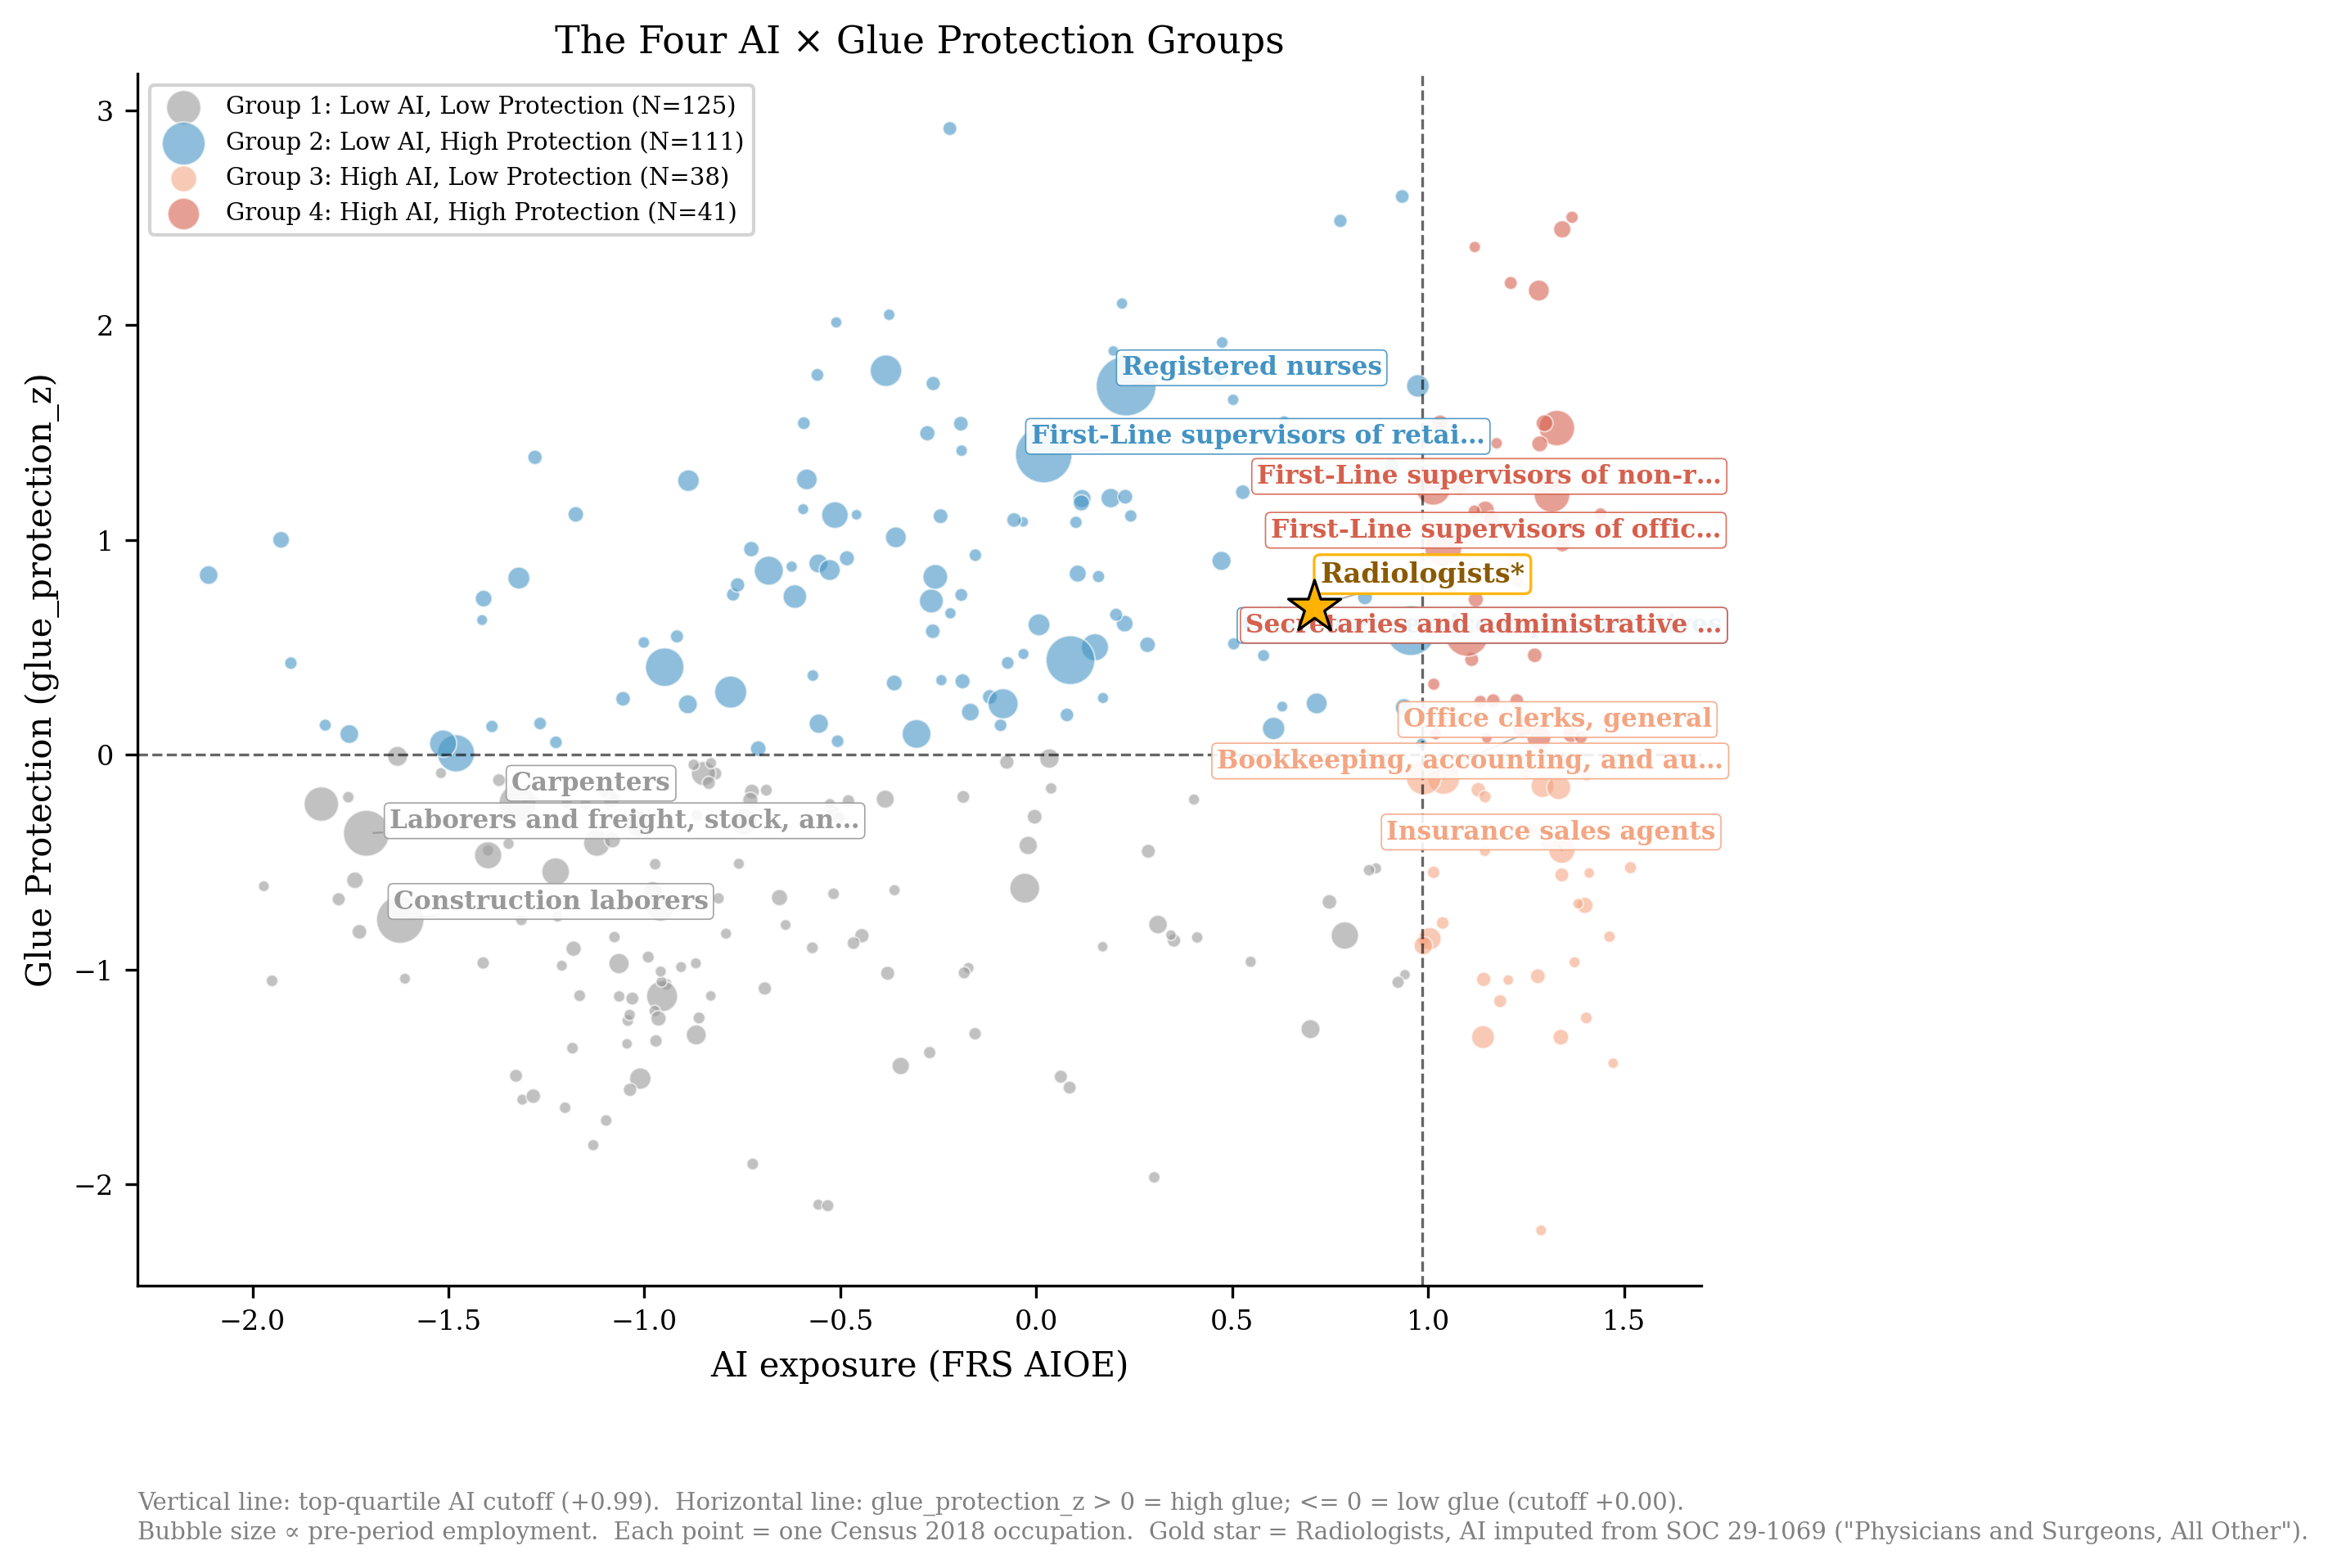
\includegraphics[height=0.6\textheight]{case5/fig_quadrants.png}
\end{center}
\end{column}
\begin{column}{0.46\textwidth}
\small\textbf{What this quadrant plot triggers.}
\begin{itemize}\scriptsize
  \item AI exposure and Glue Protection are only weakly correlated.
  \item The high-exposure column already splits into two populations.
  \item Bottom-right occupations look very different from top-right occupations.
  \item A single high-AI average would hide the mechanism.
\end{itemize}
\vspace{0.1cm}
\scriptsize
\textbf{Next move.} Compare high-protection and low-protection occupations \emph{within} the high-AI column. That request became the differential figure.
\end{column}
\end{columns}
\end{frame}

% ============================================================
% Frame 5.14 --- Headline figure
% ============================================================
\begin{frame}{The Headline Figure --- Four-Group Employment Trajectories}
\begin{center}
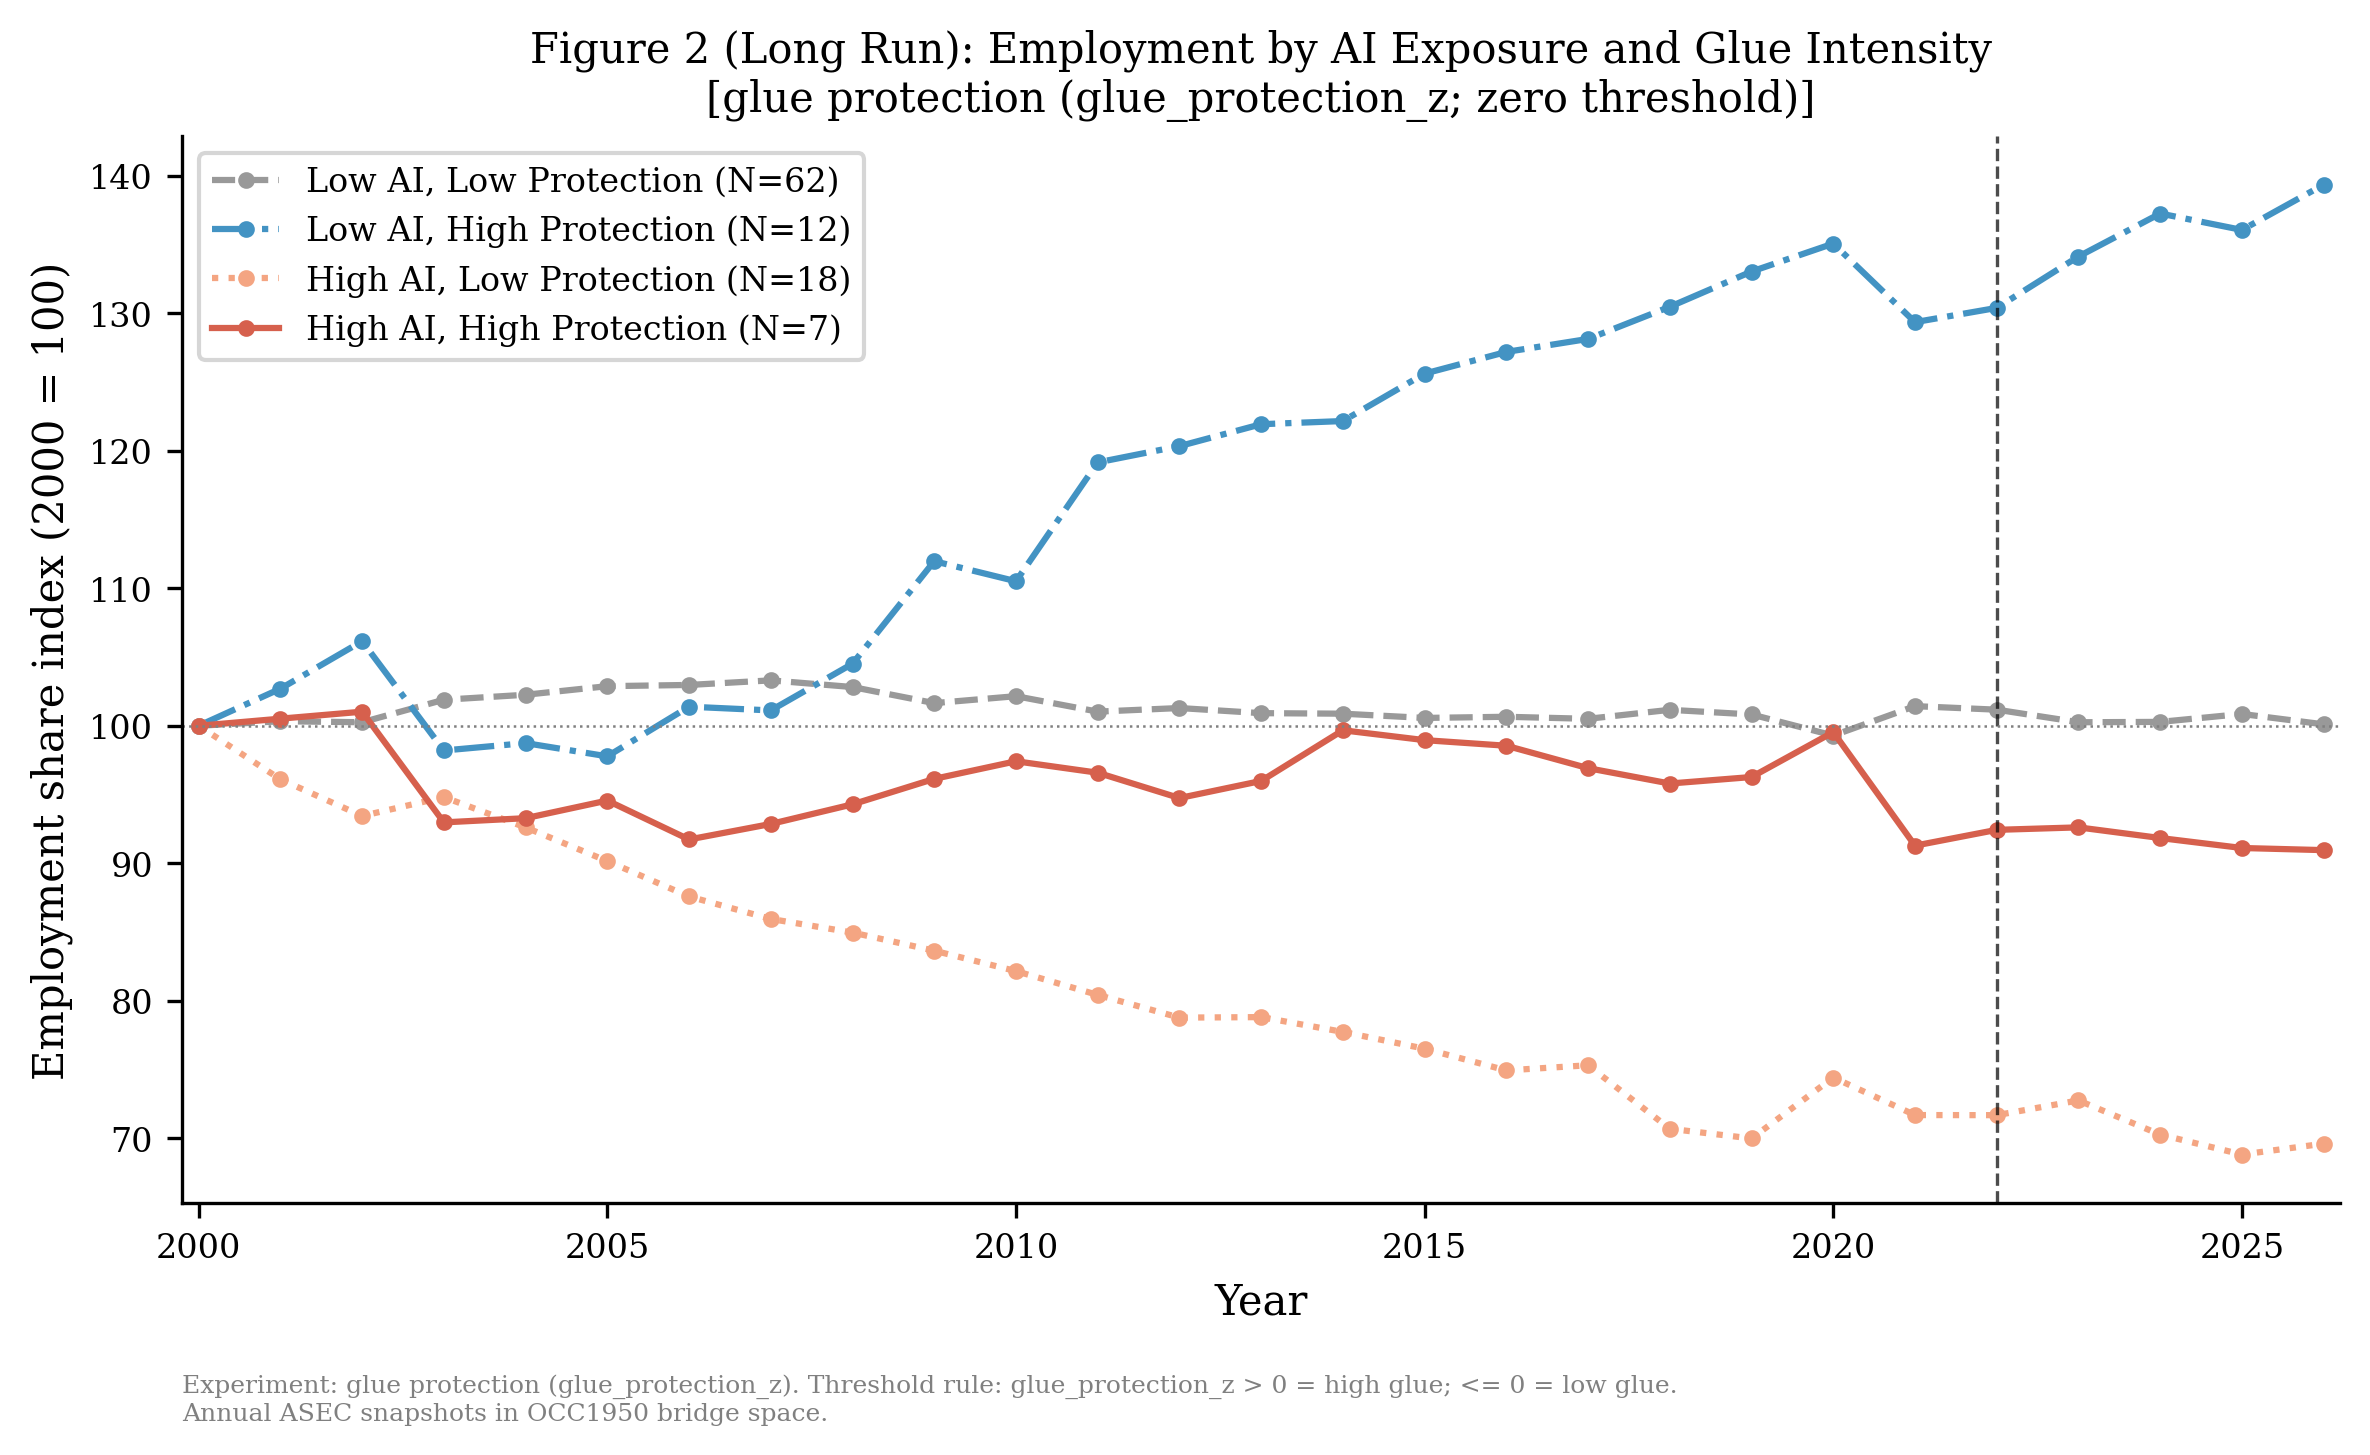
\includegraphics[height=0.66\textheight]{case5/fig_4group_trajectory.png}
\end{center}

\vspace{0.08cm}
\begin{tcolorbox}[colback=blue!3,colframe=RedTitle!60]\scriptsize
\textbf{Reading.} Once occupations are split by both AI exposure and Glue Protection, the trajectories are no longer pooled together. The theory claim is descriptive: similar AI exposure can coexist with different long-run employment paths.
\end{tcolorbox}
\end{frame}

% ============================================================
% Frame 5.15 --- Companion differential figure
% ============================================================
\begin{frame}{The Companion Figure --- Inside the High-AI Column}
\begin{center}
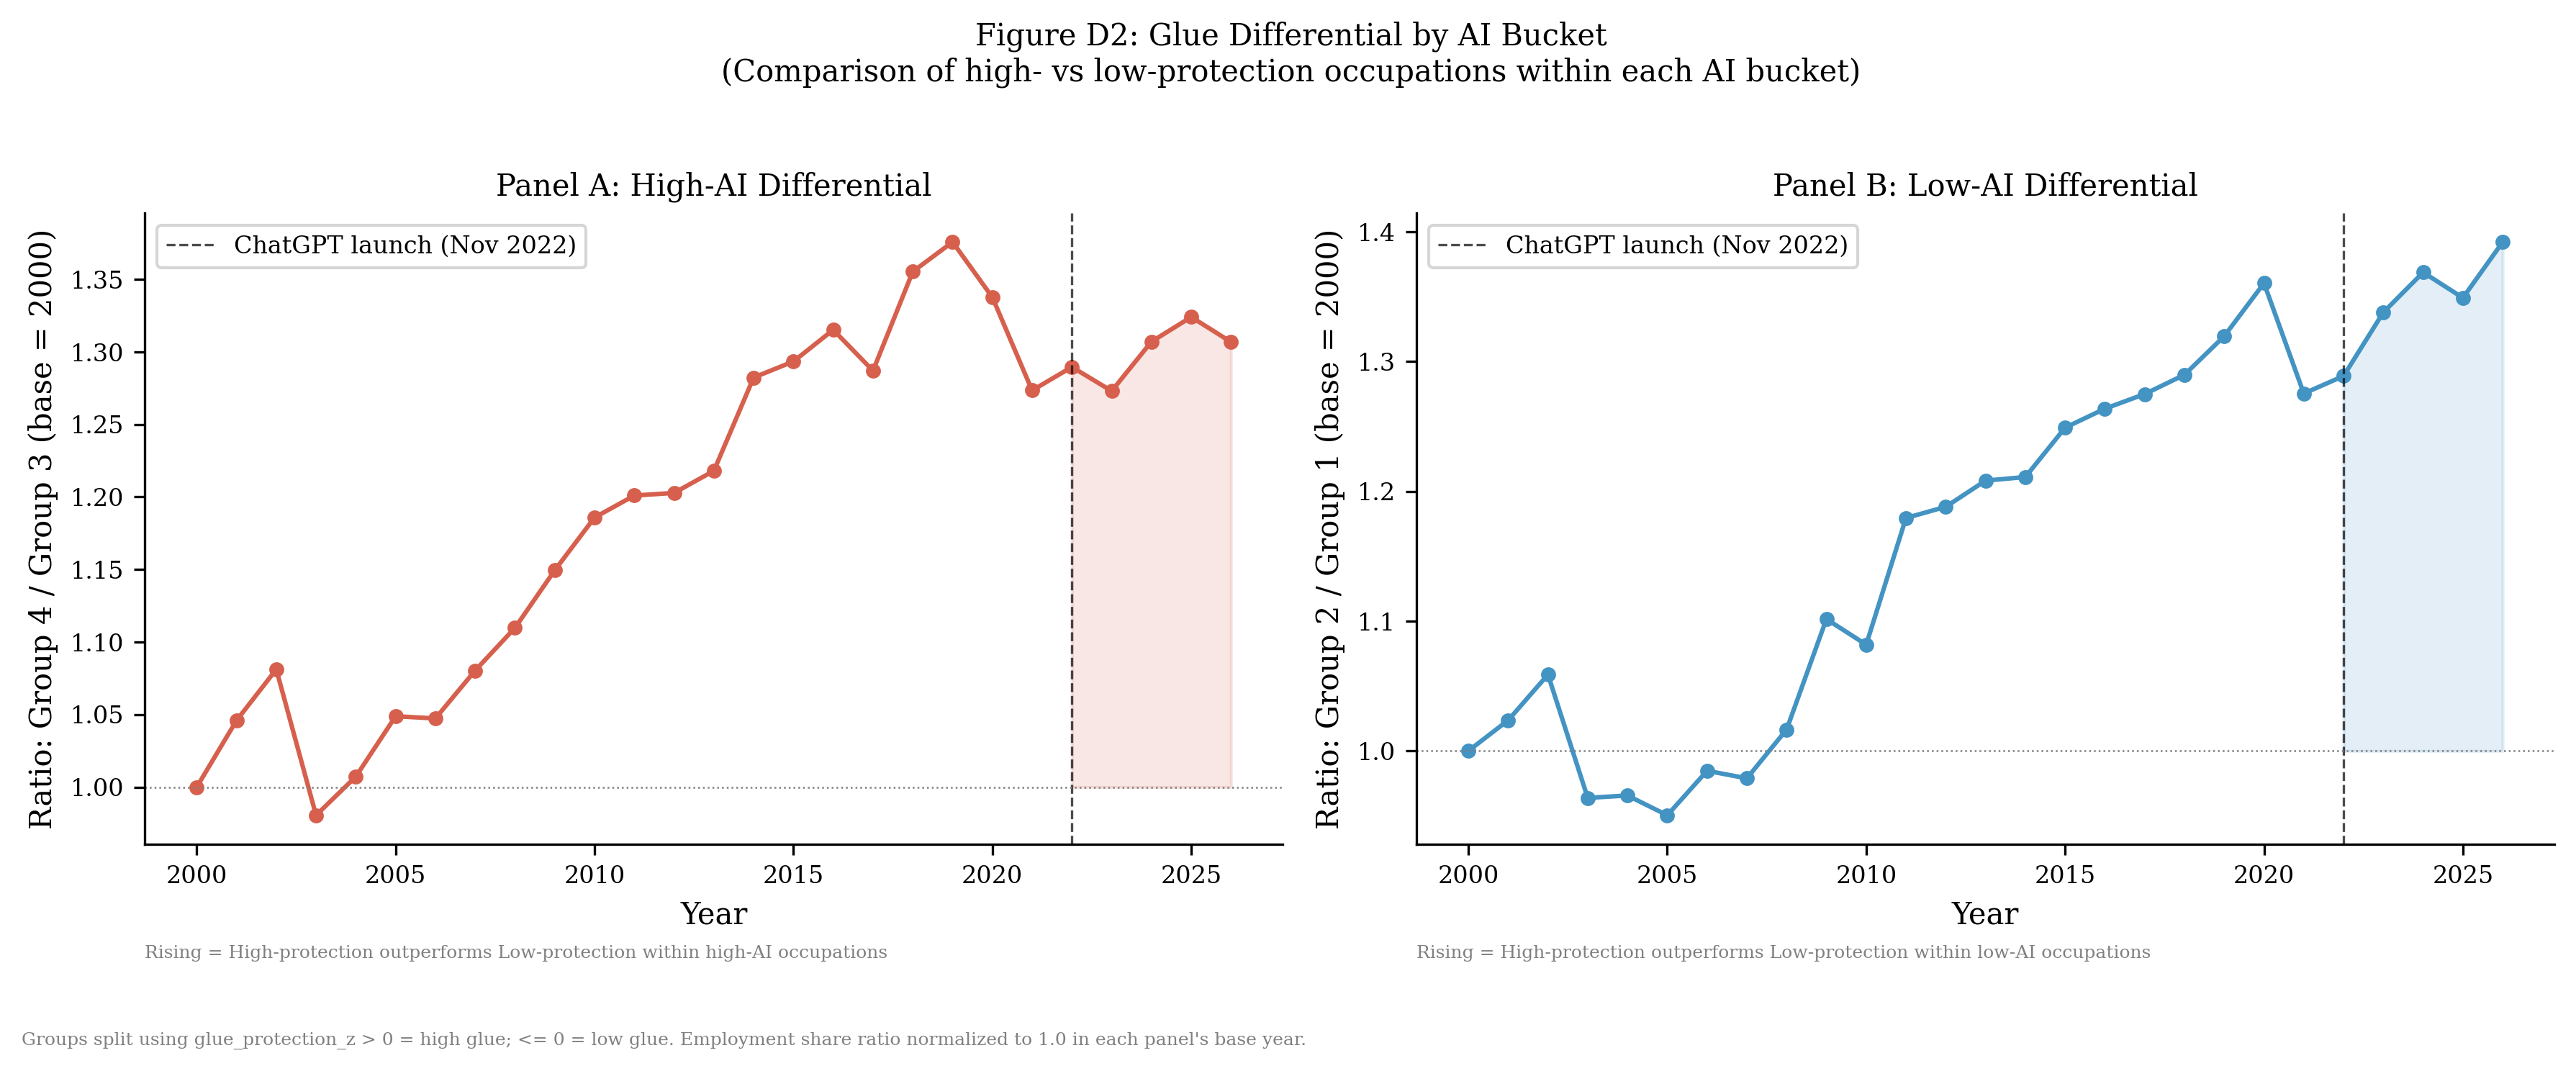
\includegraphics[height=0.68\textheight]{case5/fig_highai_differential.png}
\end{center}

\vspace{0.08cm}
\begin{tcolorbox}[colback=blue!3,colframe=RedTitle!60]\scriptsize
\textbf{Why this matters.} The ratio plot asks the cleaner question: among occupations with high AI exposure, do the high-protection occupations evolve differently from the low-protection occupations? That is the direct diagnostic behind the mechanism story.
\end{tcolorbox}
\end{frame}

% ============================================================
% Frame 5.16 --- Diagnostic Suite
% ============================================================
\begin{frame}{The Diagnostic Suite}
\scriptsize
\begin{tabular}{p{3.7cm}p{3.5cm}p{4.8cm}}
\toprule
\textbf{Diagnostic} & \textbf{What it asks} & \textbf{Where it lives (and what it found)} \\
\midrule
Management contamination & Is \texttt{glue\_core} just measuring whether the SOC prefix is ``11''? & Script 01 prints \texttt{corr(glue, is\_mgmt)} and warns when $>0.4$. \\
Sector residual (\texttt{glue\_sector\_z}) & Is glue just healthcare vs.\ production? & Partial out major-group means before re-ranking. \\
O*NET multi-wave (23.3 vs.\ 30.2) & Did task importance shift differentially in high-AI occupations? & Script 04: $\hat{\beta}_3 \approx 0$, $p\approx 0.52$. Attributed to the 2022--23 O*NET field lag. \\
Pre-trend decomposition (D1) & Is the divergence post-2022 or part of a long-run drift? & \texttt{figure\_pretrend\_allgroups\_longrun\_annual.png}: drift predates 2022. \\
\bottomrule
\end{tabular}

\vspace{0.2cm}
\begin{tcolorbox}[colback=blue!3,colframe=RedTitle!60]\scriptsize
\textbf{Rule.} Every claim in the snapshot is paired with the diagnostic that could have falsified it. The diagnostic lives on disk with a deterministic name.
\end{tcolorbox}
\end{frame}

% ============================================================
% Frame 5.15 --- Three-Document Writing Architecture
% ============================================================
\begin{frame}{Act 5 --- Three-Document Writing Architecture}
\begin{center}
\begin{tikzpicture}[
    node distance=0.4cm,
    doc/.style={rectangle, rounded corners, draw=gray!60, fill=gray!8,
        minimum width=2.9cm, minimum height=1.05cm, font=\scriptsize, text=DarkText, align=center},
    snap/.style={rectangle, rounded corners, draw=RedTitle, fill=blue!8,
        minimum width=2.9cm, minimum height=1.05cm, font=\scriptsize, text=DarkText, align=center}
]
\node[doc] (memo) {Research memo\\(62~KB, theory\\+ empirical sketch)\\\scriptsize\texttt{glue\_work\_research\_memo.md}};
\node[doc, right=of memo] (review) {Self-review\\(54~KB, six structural\\weaknesses)\\\scriptsize\texttt{critical\_review\_...md}};
\node[doc, right=of review] (design) {Design memo + review\\(31~KB + 26~KB,\\index formulas)\\\scriptsize\texttt{glue\_index\_design\_...md}};
\node[snap, right=of design] (snapshot) {Snapshot\\(6~KB, plain-English,\\for coauthors)\\\scriptsize\texttt{glue\_index\_empirical\_snapshot.md}};
\draw[->, gray!70] (memo) -- node[above, font=\tiny]{stress-test} (review);
\draw[->, gray!70] (review) -- node[above, font=\tiny]{redesign} (design);
\draw[->, gray!70] (design) -- node[above, font=\tiny]{compress} (snapshot);
\end{tikzpicture}
\end{center}

\vspace{0.15cm}
\textbf{Each step has one job.} The memo names the claim. The self-review tries to break it. The design memos rebuild the measure so the claim survives scrutiny. The snapshot delivers the survivor to a coauthor in one page. Writing one document for all four purposes produces a paper that defends everything badly.
\end{frame}

% ============================================================
% Frame 5.16 --- From Memo to Snapshot
% ============================================================
\begin{frame}{Refining --- From Memo to Snapshot}
\begin{columns}[T]
\begin{column}{0.48\textwidth}
\textbf{Memo opener} (argumentative, for the reviewer)
\begin{tcolorbox}[colback=gray!5,colframe=gray!40]
\scriptsize
A central question in the economics of AI is whether and how artificial intelligence displaces workers. Garicano, Li, and Wu (2026) push back \dots by arguing that labor markets price \emph{jobs}, not isolated tasks. \dots This memo argues that \textbf{glue work} is the missing microfoundation for bundle strength.
\end{tcolorbox}
\end{column}
\begin{column}{0.48\textwidth}
\textbf{Snapshot bottom line} (declarative, for the coauthor)
\begin{tcolorbox}[colback=gray!5,colframe=gray!40]
\scriptsize
Two occupations can have the same AI exposure and different labor-market trajectories. The Glue Protection index is an attempt to name one dimension along which they differ. The construction is declarative and inspectable; the next question is how to rationalize the pattern.
\end{tcolorbox}
\end{column}
\end{columns}

\vspace{0.2cm}
\begin{itemize}\scriptsize
  \item Compression ratio: $\sim 62$~KB memo $\to$ $\sim 6$~KB snapshot, roughly $10\times$.
  \item Audience shift: reviewer (argue for the framework) $\to$ coauthor (inspect the data).
  \item Vocabulary shift: ``microfoundation'' $\to$ ``two occupations''; theoretical verbs $\to$ empirical verbs.
\end{itemize}
\end{frame}

% ============================================================
% Frame 5.17 --- Spotting Issues, Open Threads
% ============================================================
\begin{frame}{Spotting Issues, Naming Open Threads}
\scriptsize
\begin{tabular}{p{3.7cm}p{3.3cm}p{5.0cm}}
\toprule
\textbf{Issue} & \textbf{Where surfaced} & \textbf{Disposition} \\
\midrule
Bartik shock infeasible & Act 2 data scan (BTOS Q7 suppressed at sector) & deferred; wait for a richer AI-adoption panel \\
\texttt{glue\_core} contaminated by LLM-easy items & Apr 15 self-review & \texttt{glue\_aihard\_z} promoted to co-primary; \texttt{glue\_aieasy\_z} added as penalty \\
Coordination-presence vs.\ dominance & Apr 17 review & \texttt{glue\_dominance\_z} added (mean glue $\div$ mean 41 activities) \\
Webb (2020) not integrated & crosswalk triage (occ1990dd $\to$ Census 2018 not built) & parked as robustness; waits on a new crosswalk \\
O*NET multi-wave null ($\hat\beta_3\approx 0$) & Script 04 diagnostic & attributed to 2022--23 field lag; rerun on O*NET 31 when released \\
\bottomrule
\end{tabular}

\vspace{0.2cm}
\begin{tcolorbox}[colback=blue!3,colframe=RedTitle!60]\scriptsize
Each row is where the next sprint starts. A sprint that ends without a written issue list starts the next sprint by rediscovering its own unsolved problems.
\end{tcolorbox}
\end{frame}

% ============================================================
% Frame 5.18 --- Division of Labor Move by Move
% ============================================================
\begin{frame}{Division of Labor --- Move by Move}
\scriptsize
\begin{tabular}{p{3.1cm}p{4.2cm}p{4.7cm}}
\toprule
\textbf{Move} & \textbf{Agent did} & \textbf{Economist did} \\
\midrule
Name the puzzle & draft the three-sentence opener from a literature sweep & chose GLW (2026) as the anchor; named glue work as the missing microfoundation \\
Choose O*NET items & proposed five items from the content model & vetoed three LLM-easy items; added the embodied/relational list \\
Build the pipeline & wrote scripts 00--14, wired \texttt{config.py}, added 51 unit tests & locked the parameter values and the STOP GATE criterion \\
Spot sign reversal & printed the pre/post deltas; surfaced the pattern & recognised it as a theory problem, not a bug \\
Reframe theory & produced three candidate rewordings & chose reallocation-not-survival; wrote the new abstract \\
Design the four-index family & drafted \texttt{aihard}, \texttt{dominance}, \texttt{social}, \texttt{aieasy} with weights & fixed the 35/25/25/15 weights; named the composite \\
Write the snapshot & compressed 62~KB $\to$ 6~KB on request & read the draft as a coauthor would; rewrote the bottom line \\
\bottomrule
\end{tabular}

\vspace{0.2cm}
\textbf{The constant.} The agent executes; the economist decides what is true. The economist's work is not replaced --- it is concentrated into judgment calls.
\end{frame}

% ============================================================
% Frame 5.19 --- End of Stage 1: Memo + Coauthor Discussion
% ============================================================
\begin{frame}{End of Stage 1 --- Memo, Critique, and What Triggered Stage 2}
\begin{columns}[T]
\begin{column}{0.32\textwidth}
\textbf{The memo (6 KB)}
\begin{tcolorbox}[colback=gray!5,colframe=gray!40]\scriptsize
\emph{``Two occupations can have the same AI exposure and different labor-market trajectories. Glue Protection names one possible reason. The construction is inspectable; the next step is to explain the pattern.''}
\end{tcolorbox}
\scriptsize One page, plain English, readable by a coauthor in three minutes.
\end{column}
\begin{column}{0.32\textwidth}
\textbf{The coauthor critique}
\begin{tcolorbox}[colback=gray!5,colframe=RedTitle!60]\scriptsize
\textbf{Apr~18 critique:}
\begin{itemize}\scriptsize
  \item ``You're still using the mean of a within-occupation distribution. The \emph{shape} matters.''
  \item ``If two tasks have very different exposures, the job gets \emph{unbundled} --- not \emph{substituted}.''
  \item ``Add a second measure: how dispersed is the exposure \emph{within} an occupation?''
\end{itemize}
\end{tcolorbox}
\end{column}
\begin{column}{0.32\textwidth}
\textbf{The question that launched Stage 2}
\begin{tcolorbox}[colback=blue!3,colframe=RedTitle!60]\small
\emph{Holding mean AI exposure fixed, does within-job dispersion of exposure predict labor-share outcomes?}
\end{tcolorbox}

\vspace{0.12cm}\scriptsize
That question became the Stage 2 workflow over the next week.
\end{column}
\end{columns}

\vspace{0.12cm}
\begin{tcolorbox}[colback=blue!3,colframe=RedTitle!60]\scriptsize
\textbf{Rule.} A short memo plus an honest critique is the cheapest way to make the next sprint smarter.
\end{tcolorbox}
\end{frame}

%===========================================================

\end{document}
